\section{SAND}\label{sec:sand}

In this section, we introduce the main ideas behind SAND, describe our implementation for Nuclio and the components in detail, and compare our implementation to that of Akkus et al.~\cite{akkus2018sand}.

\subsection{Concepts}

When building serverless applications, it is important to connect the invocations of different functions into function chains or workflows.
Because FaaS-platforms often host functions of different applications for different users, providing isolation between functions is a critical issue.
It should not be possible for a function to access the data of functions deployed by other users, for example.
At the same time, functions of the same application typically requires less isolation between each other than functions of different applications.
Akkus et al.~refer to this idea as \enquote{two-level fault isolation}~\cite{akkus2018sand}.
In turn, reducing isolation between functions (of the same application) can lead to performance improvements.
Instead of trying to optimize individual functions, we can reduce the total workflow duration by reducing the latency between steps of a workflow.
Similarly, allowing different functions to access shared data can improve the platform's resource usage. 

To demonstrate these ideas, Akkus et al.~present SAND~\cite{akkus2018sand}.
SAND is a serverless platform that aims at improving application performance by reducing the isolation between functions of the same application.
Figure~\ref{fig:sand_architecture} shows an overview of SAND's architecture.
The platform consists of the following components.
\begin{itemize}
    \item \emph{Grain}: A grain is an individual FaaS function.
    \item \emph{Application}: An application is a set of functions and the workflows defined for these functions. It can span across multiple hosts.
    \item \emph{Sandbox}: An application has its own container on a host, which is the sandbox. 
    \item \emph{Message bus}: A message bus is a means for functions of the same application to communicate. 
    \item \emph{Grain worker}: A grain worker is a function worker. It loads the function code and its dependencies, subscribes to the grain's queue, and invokes the function accordingly.
\end{itemize}

\subsubsection{Application Sandboxing}\label{subsub:application_sandboxing}

\begin{figure}
    \centering
    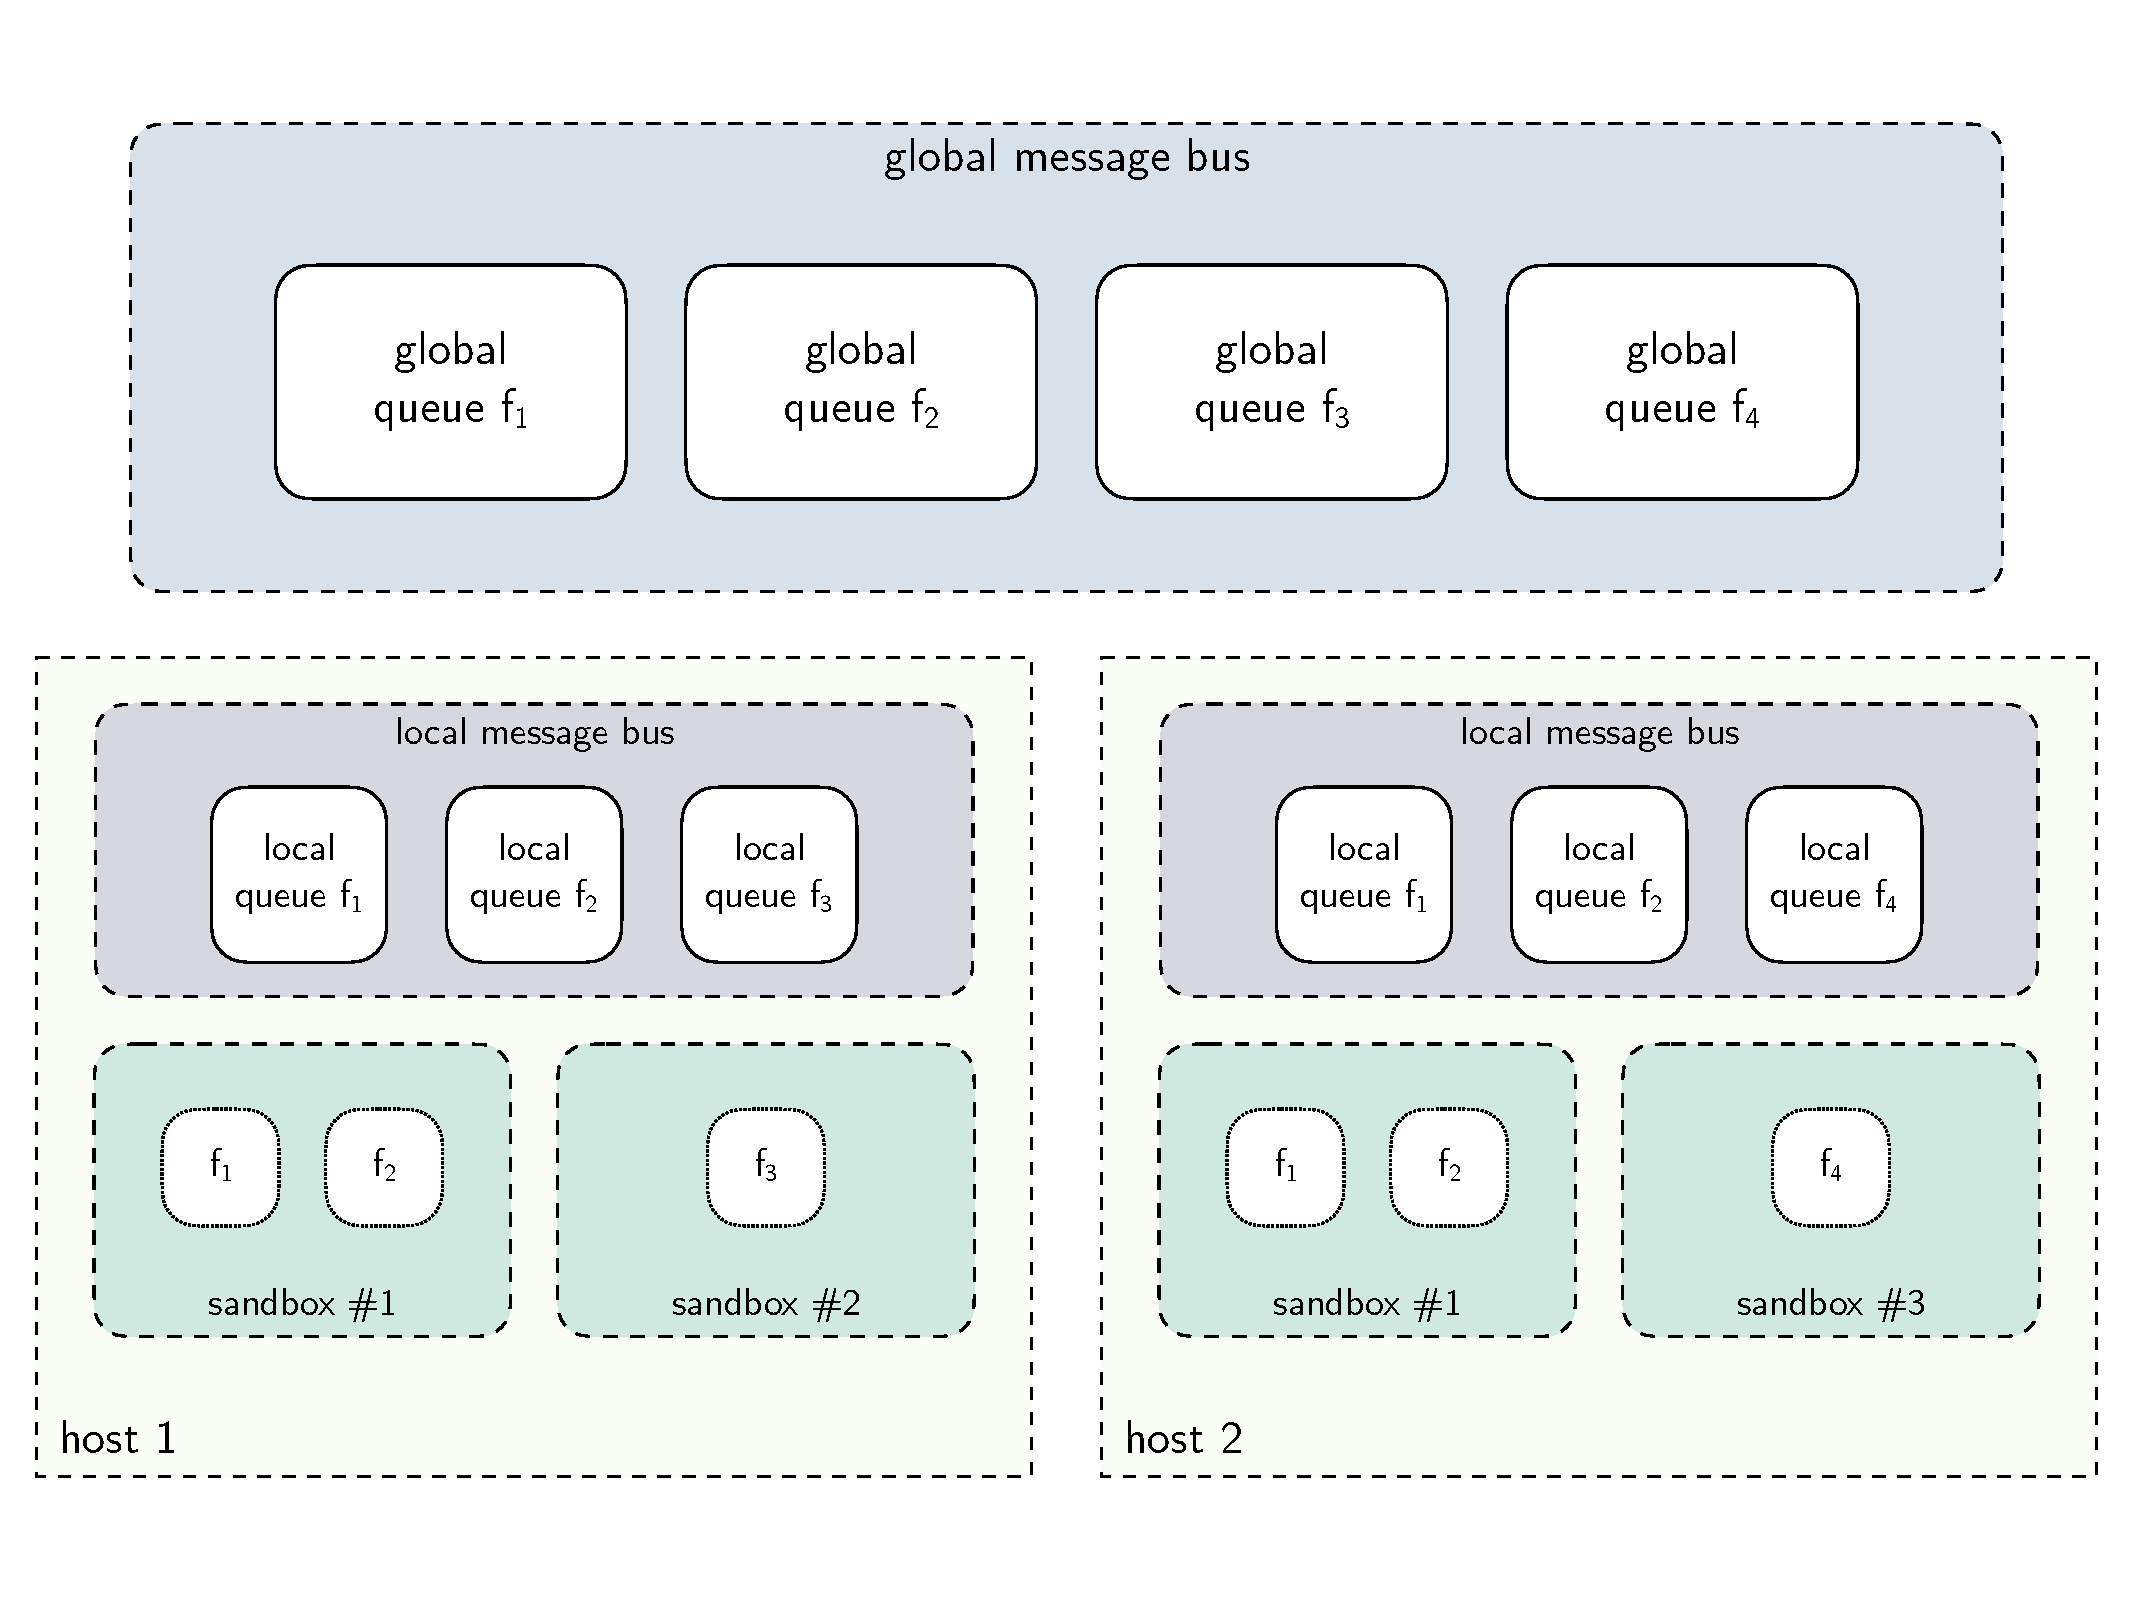
\includegraphics[width=\linewidth]{figures/sand_architecture.pdf}
    \caption{
        SAND's architecture comprises multiple hosts, multiple applications spanning across multiple hosts, sandboxes on the hosts containing different functions in addition to a local message bus, and a global message bus~\cite{akkus2018sand}.
    }\label{fig:sand_architecture}
\end{figure}

In order to realize these benefits while keeping isolation between functions of different applications, Akkus et al.~introduce \enquote{application sandboxing}~\cite{akkus2018sand}.
They list different technologies and options for implementing two-level fault isolation, among which are VMs, containers, unikernels, processes, and threads.

SAND uses Docker containers for their sandbox implementation~\cite{akkus2018sand}.
Each application runs in a different container, and the functions making up the applications run as different processes.
To handle incoming requests, SAND uses process forking.
The benefits of this approach are threefold.
\begin{itemize}
    \item The startup latency using process forking is far lower than the startup latency using new containers for function invocations.
    \item Libraries shared by functions only need to be loaded once in an application.
    \item Memory use increases only slightly with new function invocations, and the memory is released immediately once the function call is over, which leads to more efficient resource usage.
\end{itemize}

\subsubsection{Hierarchical Message Queuing}

To implement a workflow in a serverless platform that does not explicitly provide means of function chaining, functions typically invoke the workflow's next step by sending requests to the platform in the same way an external invocation would be sent.
This is inefficient from both the perspective of the platform and of the workflow developer.
For the platform, this creates additional load as internal requests compete for resources with external requests at the platform's gateway.
For the workflow developer, this adds potentially high latency between function calls, which increases the total workflow duration and end-to-end latency, in turn.

SAND can run in a distributed manner across multiple hosts.
In addition, it is possible for an application to span multiple hosts.
For example, the application could consist of more functions than a single SAND host can handle, or the application might be distributed across multiple regions with improved function placement.
Consequently, functions of the same application need to be able to communicate with other functions running on the same and on different hosts.

As SAND treats internal and external requests differently, it provides two additional options for functions to communicate.
This allows SAND to have \enquote{shortcuts for functions that interact with each other}~\cite{akkus2018sand}.
\begin{itemize}
    \item The \emph{local message bus} allows functions in the same sandbox to communicate.
    \item The \emph{global message bus} handles invocations across hosts and serves as backup for the local message buses.
\end{itemize}
Here, a message bus is a set of FIFO queues, containing one queue per function, where each messages in a queue corresponds to a function call.

\subsection{Implementation Overview}

Akkus et al.~implemented SAND using Docker containers for application sandboxing~\cite{akkus2018sand}.
To implement a similar feature for Nuclio, we need to adapt their design to fit better for Nuclio's design.
Nuclio offers two backends for deploying functions: Docker and Kubernetes, where the Docker backend is intended for development purposes and the K8s backend for production. 
Therefore, the SAND implementation for Nuclio should reflect the focus on Kubernetes.

While using the Kubernetes backend, Nuclio deploys a new pod for each function, which contains only one container for the function processor, respectively.
Using the same abstraction level as SAND—as in using containers for application sandboxing—does not reflect Nuclio's use of Kubernetes well, and it seems infeasible given the scope of Nuclio's codebase. 
Taking this into account, we choose Kubernetes pods as our means of application sandboxing.

% TODO maybe remove the arrows
\begin{figure}[!h]
    \centering
    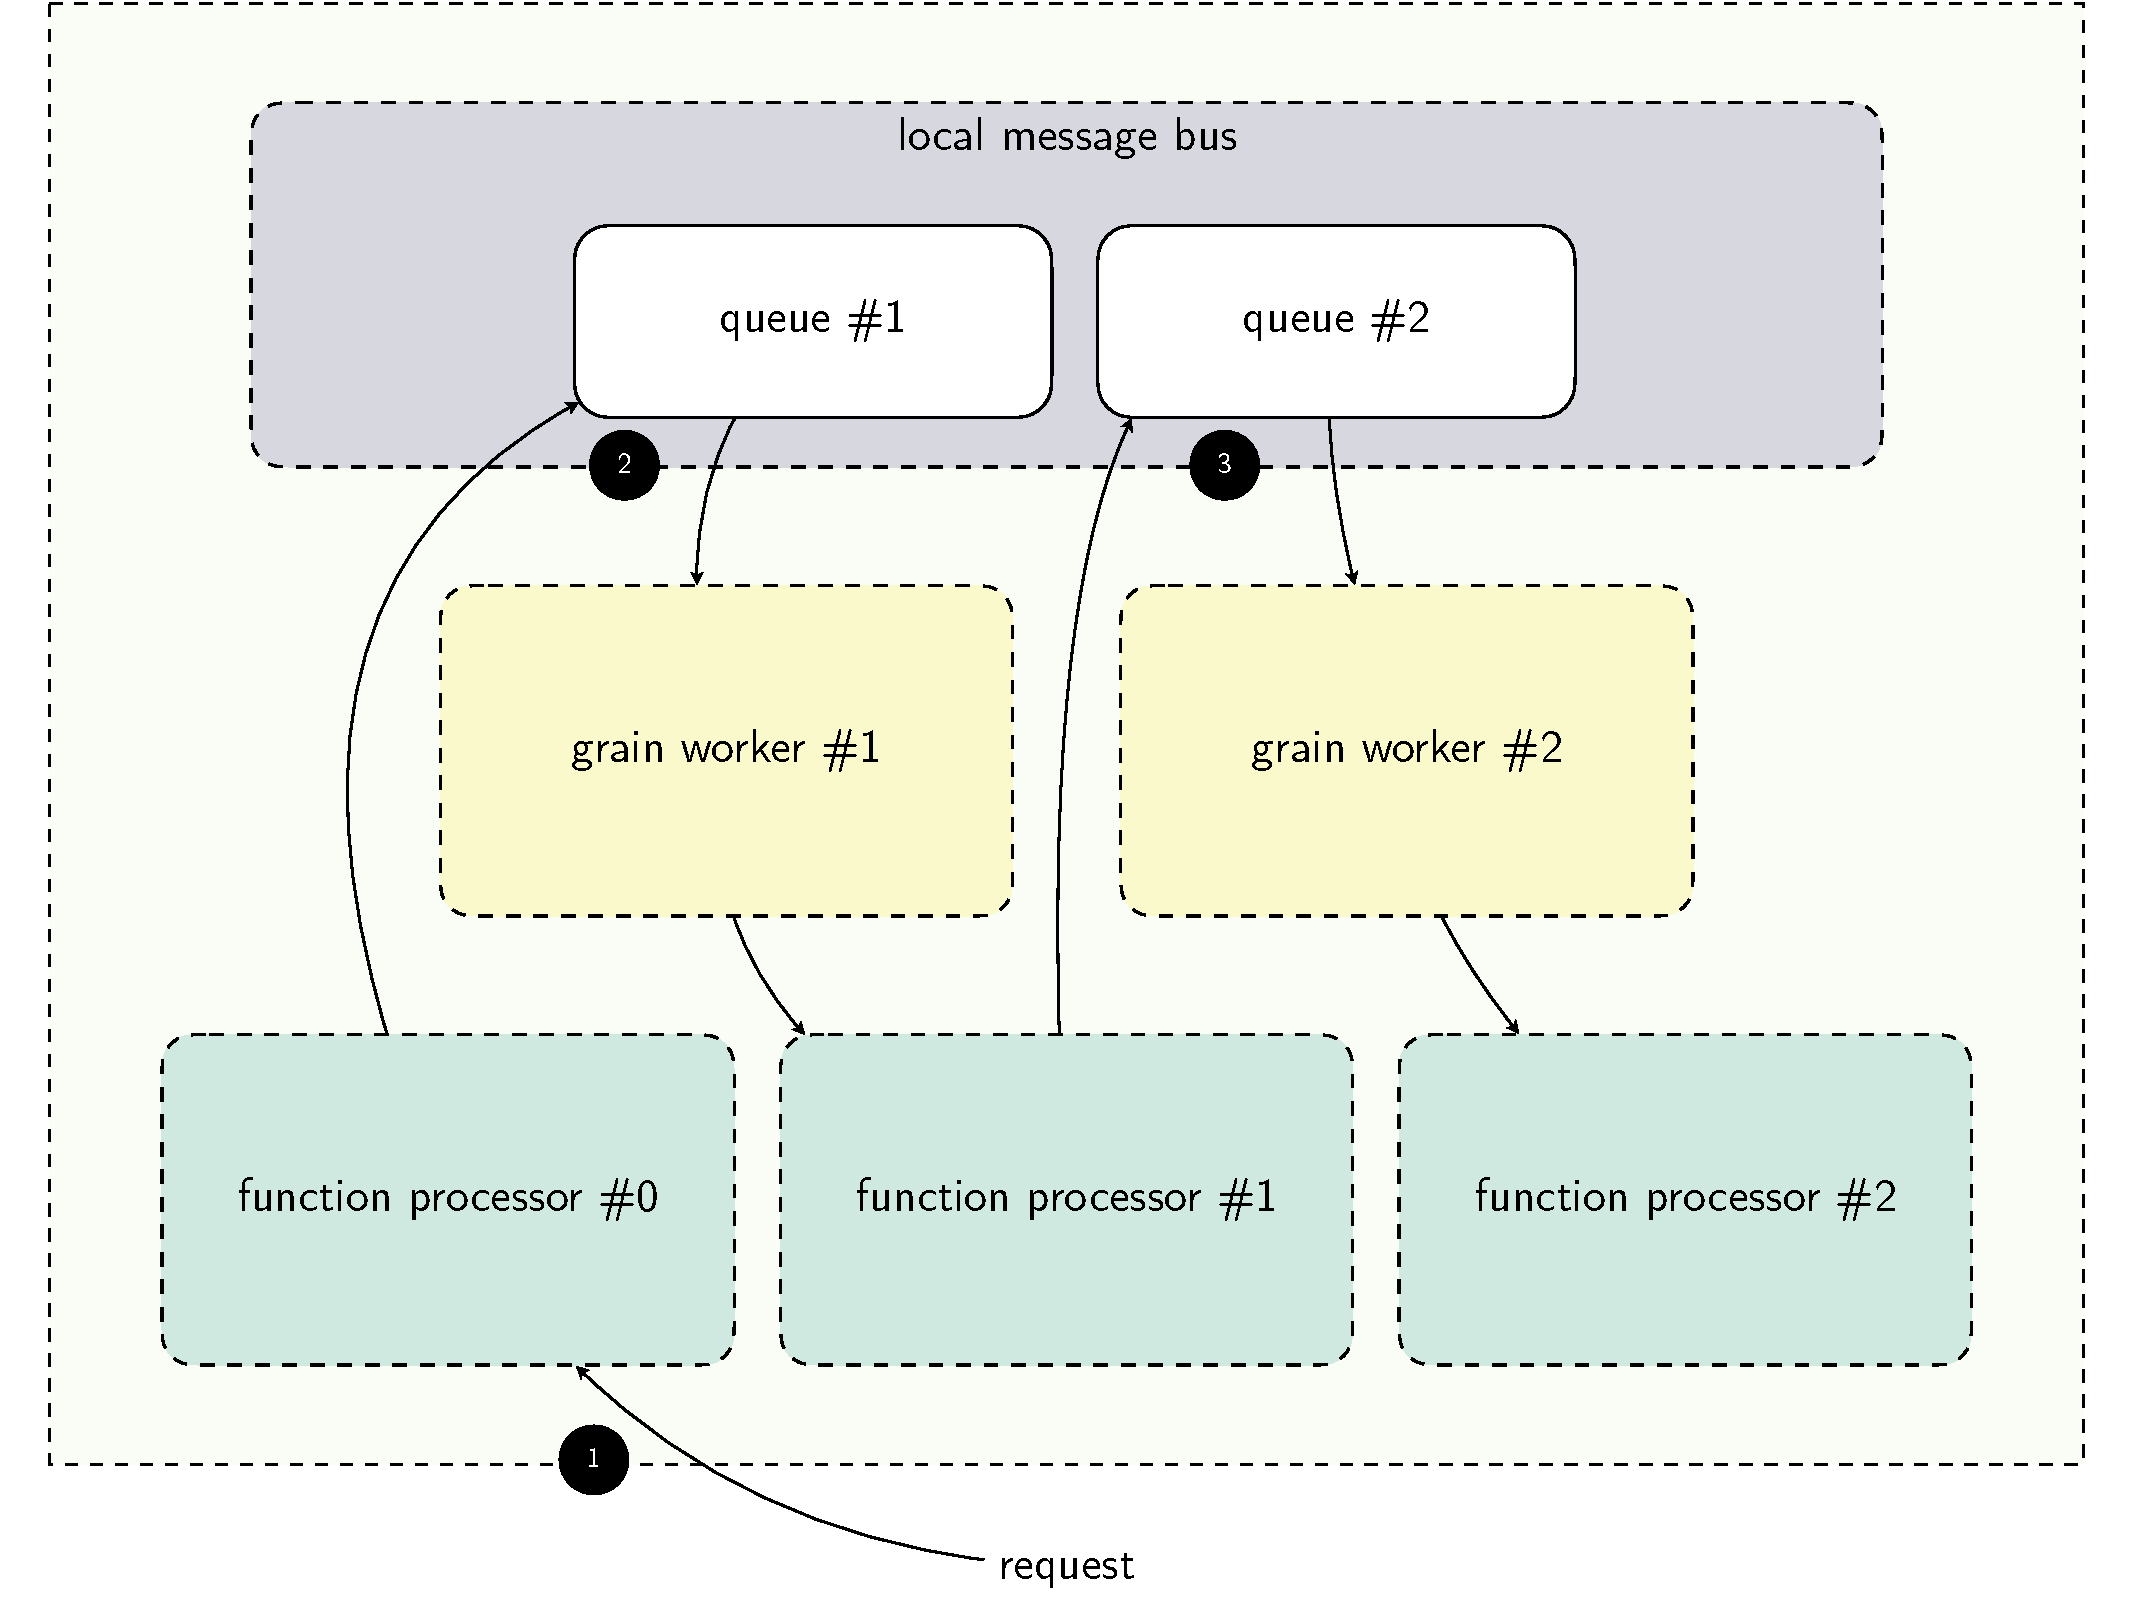
\includegraphics[width=\linewidth]{figures/sandbox.pdf}
    \caption{
        Our implementation of application sandboxing in Nuclio uses Kubernetes pods for isolation and contains containers for function processors, grain workers, and a local message bus. 
        Workflow steps are invoked by sending messages to the local message bus, which the next grain worker receives and uses to invoke its function.
    }\label{fig:sandbox}
\end{figure}

This way, our implementation merges Nuclio's function pods to create application sandboxes. Figure~\ref{fig:sandbox} shows an overview of our sandbox design, which contains $n$ containers for different function processors, $n-1$ containers for the grain workers, and a single container for the local message bus.

To invoke other functions, a function sends an AMQP message to the local message bus (which it can reach at \texttt{localhost:5672}). 
The queues have the same name as the functions for which they process requests, and the messages contain the function inputs. 
This allows the actual workflows to be determined dynamically at runtime depending on the functions' logic and their inputs.

Figure~\ref{fig:sandbox} also shows the general workflow process in the sandbox. 
\begin{enumerate}
    \item First, the Nuclio dashboard forwards an (external) request to the sandbox, where it is received directly by the workflow's first function. 
        The function is invoked, after which it invokes the next step by sending a message to queue corresponding to the workflow's next step.
    \item Next, the second function's grain worker—which is subscribed to \texttt{queue \#1}—receives the message and invokes its function.
        Again, the function is invoked, and it sends a message \texttt{queue \#2} after it has finished.
    \item Last, the second grain worker receives the message for the last step.
        It invokes its function, which concludes the workflow.
\end{enumerate}

When using the K8s backend, Nuclio can be distributed across multiple nodes, similarly to how SAND uses multiple hosts.
For implementing workflows across hosts, the Nuclio dashboard can be used as the global message bus. 
When calling functions of the same application in a different sandbox, the request is sent to the dashboard, which forwards it to the correct function.

\subsection{Components}

Next, we go over the different components of our implementation in more detail and highlight some differences to SAND.

\subsubsection{Sandbox}\label{subsub:sandbox}

In our implementation, a sandbox corresponds to a Kubernetes pod. 
Consequently, an application is a set of pods that run on different nodes, where the functions communicate through their local message bus or the Nuclio dashboard, depending on the location of the next function.

When deploying a function to its K8s backend, Nuclio creates a new \texttt{deployment} (which is a Kubernetes resource).
We modify this deployment to create custom application sandboxes.

To create a sandbox, we first require Docker images for the Nuclio function processors, as well as for the grain workers and local message bus.
Images for the function processors can be created using the builder that is accessible through the dashboard. 
As part of using Nuclio's K8s backend, we create a Docker registry that is used to push and pull Docker images for deploying new functions.
The images for the function processor have to be pushed into this registry.
In addition, we build a docker image for the grain workers and an image for the local message bus, which also have to be pushed to the registry.

Next, we modify the deployment configuration created for the workflow's first step to include all other components of the sandbox.
It is important to note that we have to modify the \emph{deployment} instead of, for example, the pod configuration. 
Otherwise, K8s will not add any additional containers to the previously created pod.
To add the additional containers to the pod, we list them under \texttt{spec.template.spec.containers} in the deployment configuration.
Here, we also set the ports and environment variables for the containers. 
The ports we set for the containers have to be unique; in K8s, \texttt{localhost} always refers to a pod.
Since containers in the same pod share their network space, networking between them becomes easier, but the ports used cannot overlap across containers.
For setting up the grain workers, we set the environment variables \texttt{FUNCTION\_NAME} and \texttt{FUNCTION\_PORT} to point to their respective function. 
It is also noteworthy that this approach to building sandboxes makes our SAND implementation compatible with our ProFaaStinate implementation.
To the Nuclio dashboard, it appears that the sandbox is a normal Nuclio function pod, and it starts the workflow as it would invoke any other function. 
Since our ProFaaStinate implementation modifies the Nuclio dashboard to allow asynchronous (and, consequently, the scheduling of) requests, the \emph{start} of the workflow can be delayed, too.

\subsubsection{Grain}

A grain is represented by a Nuclio function processor. 
For our use case, the grain carries the user's function, listens to HTTP requests, and invokes the function accordingly.
More general information on Nuclio's function processor can be found in
section~\ref{sec:nuclio}. % TODO TODO TODO

Nuclio's function processors contain workers to execute the user's code and different triggers to listen for requests.
We modified the HTTP trigger to be able to configure on which port it listens for HTTP requests inside the port using the environment variable \texttt{SAND\_PORT\_INTERNAL}.
Because of the intra-pod networking outlined above, function processors for different functions in the same pod cannot bind to the same ports, which made this change necessary.


\subsubsection{Grain Worker}

The grain workers are implemented as a Docker container running Alpine Linux 3.19\footnote{https://www.alpinelinux.org/} and Golang 1.21.4\footnote{https://go.dev/}.
When started, a grain worker looks for the environment variables set earlier (see~\ref{subsub:sandbox}) and subscribes to the respective queue at the local message bus.
If the queue does not yet exist, it is created by the grain worker.
For each message it receives from the local message bus, it sends an HTTP request to the correct function processor in order to invoke the function.

Within the sandbox, there exist $n$ grains and $n-1$ grain workers.
Since the workflow's first function is invoked directly by the request from the dashboard, there is no need for an additional grain worker for the first function.
Cyclic workflows could pose an exception to this; however, the sandbox' configuration can be easily adapted to fit this use case.

\subsubsection{Local Message Bus}

The local message bus is implemented a Docker container running Ubuntu 22.04 LTS\footnote{https://releases.ubuntu.com/jammy/}.
This container runs RabbitMQ, which we use as the message bus. 
We chose to use Ubuntu as the base image even though there is a RabbitMQ Docker image because the image is only community-maintained and less stable in our experience.
Conversely, using Ubuntu allows us to use the APT package \texttt{rabbitmq-server}, which is one of the recommended options\footnote{https://www.rabbitmq.com/docs/install-debian} for installing the message broker.

The container exposes the port 5672 to receive AMQP messages and 15672, which allows us to access RabbitMQ's management interface (with port forwarding). 

In the local message bus, there is one queue per function in the sandbox.
The queues are created automatically with the start of the grain workers. 
As part of AMQP, RabbitMQ has exchanges, where it received messages, and queues, to which the received messages are routed and from where it sends messages to any subscribed consumers.
For all messages, we use the default exchange.


\subsection{Differences to Akkus et al.'s Implementation}

Our implementation of application sandboxing and hierarchical message queuing differs in three ways from the implementation of Akkus et al.'s SAND~\cite{akkus2018sand}.
% 1 technologies
% 2 abstraction level for sandboxes
% 3 beginning of workflow process

\paragraph{Technologies}

Akkus et al.~\cite{akkus2018sand} use different technologies to implement their components. 
First, their prototype is implemented in Java and Python, while we use Golang as Nuclio is implemented in Golang.
Next, they use Apache Kafka for the global message bus and a custom Java-implementation for the local message bus, while we use RabbitMQ as Nuclio already offers a tech-preview for supporting RabbitMQ, which made it a good fit for the local message bus.\footnote{https://nuclio.io/homepage/rabbitmq/} 
In our implementation, we use the Nuclio dashboard as the global message bus.
In addition, SAND uses Apache Cassandra and NGINX.

\paragraph{Sandbox}

The next difference is in the level of abstraction for the implementation of application sandboxing.
In SAND, an application sandbox is implemented as a Docker container, while we use Kubernetes pods to this end. % TODO formulierung
Even though using containers leads to better performance by making communication between functions more direct, using pods instead fits better given Nuclio's use of Kubernetes.
Further, using containers for sandboxing would have required a near re-write of the function processors, which was infeasible with regard to the scope of the project. % TODO vielleicht lieber raus?

\paragraph{Workflow Process}

The last and smallest difference lies in the beginning of the workflow process. 
In SAND, after a request reaches the platform, the load balancer forwards it to the global message bus, where a grain worker handles it.
In contrast, requests go directly from the dashboard to the workflow's first function in our implementation.
The reason for this difference is that the Nuclio dashboard serves as load balancer and global message bus in our system.

\subsection{Limitations and Possible Improvements}

Our implementation has the following limitations.

\paragraph{Data Layer}

In addition to the hierarchical message queuing, the SAND platform also has a data layer, which allows the sharing of references to data instead of transferring the actual data between functions.
This data layer did not serve a large purpose in our project, as the implementation of application sandboxing and hierarchical message queuing in Nuclio was motivated by the comparison of total workflow durations of workflows between Fusionize and SAND.
However, adding this data layer does not pose a large challenge: In SAND, the (local) data layer is a key-value store \enquote{runs on each host similar to the local message bus}~\cite{akkus2018sand}.
In order to add this to our implementation, a key-value store can be added as an additional container inside an application's pod, which enables the same functionality. 

\paragraph{Pods as Sandboxes}

Using Kubernetes pods as sandboxes comes with a performance penalty, compared to other options listed in~\ref{subsub:application_sandboxing}.
This is to be expected, as Kubernetes pods are a significantly larger unit for sandboxing than, for example, using unikernels; however, it is still the best-fitting choice given Nuclio's design.

\paragraph{The Nuclio Dashboard}

Given that the Nuclio Dashboard treats the sandbox as a single function, we are not able to access other functions in the application with external requests. 
This is negligible for many use cases, where the start of the workflow is fixed, but this is still improvable.

\paragraph{Possible Improvement: Grain Workers}

A possible improvement is the direct integration of the grain workers into the function processors. 
The grain workers and the function processors' triggers serve a similar purpose: listen to events and invoke the function accordingly.
Currently, Nuclio offers a tech-preview for RabbitMQ triggers, indicating that improved support for the message broker can be expected in the future.
Once this is rolled out, the function processor could be configured to listen to the local message bus directly, which would make communication more direct and likely improve total workflow duration. 
However, this is only possible once Nuclio offers better support for RabbitMQ (or another event trigger), as is it not stable enough, yet.
